\documentclass[tikz,border=2pt]{standalone}

\usepackage{xcolor}

% Roughly match the three fill colors
\definecolor{regionA}{rgb}{0.83,0.60,0.31} % brownish
\definecolor{regionB}{rgb}{0.34,0.55,0.75} % blue
\definecolor{regionC}{rgb}{0.34,0.45,0.53} % blue-gray

\begin{document}
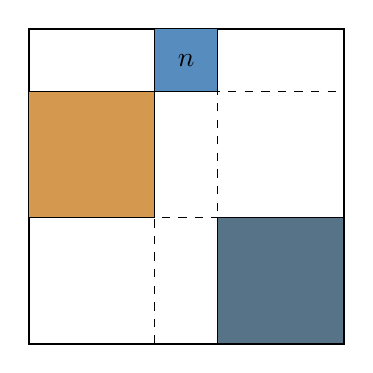
\begin{tikzpicture}[scale=0.8]

  % Outer square
  \draw[thick] (0,0) rectangle (5,5);

  % Dashed subdivision lines
  % (ratios chosen to match the SVG: widths 2:1:2, heights 2:2:1)
  \draw[dashed] (0,2) -- (5,2);
  \draw[dashed] (0,4) -- (5,4);
  \draw[dashed] (2,0) -- (2,5);
  \draw[dashed] (3,0) -- (3,5);

  % Filled regions (same relative positions as in the SVG)
  % Left–middle block
  \filldraw[regionA,draw=black] (0,2) rectangle (2,4);

  % Top–middle thin block
  \filldraw[regionB,draw=black] (2,4) rectangle (3,5);

  % Bottom–right block
  \filldraw[regionC,draw=black] (3,0) rectangle (5,2);

  % Optional label in the top middle (guessing from context)
  \node at (2.5,4.5) {$n$};

\end{tikzpicture}
\end{document}
